\chapter{Results}
This section details the experimental results of investigating the effect of strain in $^{171}$Yb doped YSO. Following each cool down and prior to any pulse measurement the centre frequency $f_{c}$ of the cavity is obtained in tunning mode. Tunning mode is the safety setting in which the signal always bypasses the LNA. The cavity resonance is differentiated from electronic reflections by tunning the cavity Q factor and observing which absorption peak changes in width. The VSG is set such that the output pulse is resonant with $f_{c}$, where $f_{c}\approx 6.3$ GHz. The Q factor is tuned as required. Thereafter, in pulse mode the attenuation of the input is slowly decreased whilst the ensuring there is no pulse ringing in the acquisition window. 


\section{EPR setup testing}
Following the re-installment of EPR equipment a Gauss meter, measuring up to 30 mT, was used to test the accuracy of the low magnetic fields generated by the field controller. To test the functionality of the setup, EPR spectroscopy of a P doped isotropically purified $^{28}$Si sample was initially completed at 9 K. The strength of echo signal above the noise floor for this sample reduced the difficulty of finding the resonance field for a transition. However, for a Rabi pulse sequence, where the initial pulse duration was swept, the signal amplitude never recovered to complete Rabi oscillations as shown in Fig.~\ref{fig:rabisi28}. Regardless of the settings of the pulse sequence and acquisition time the oscillations were not observed. Additionally a significantly shorter $T_{1}$ time of the order of ns was obtained whilst previous experimental measurements the longitudinal electron spin relaxation time determined this should be of the order of ms~\citep{PhysRevB.68.193207}.  

\begin{figure}[H]
    \centering
    \begin{subfigure}[b]{0.45\textwidth}
        \centering
        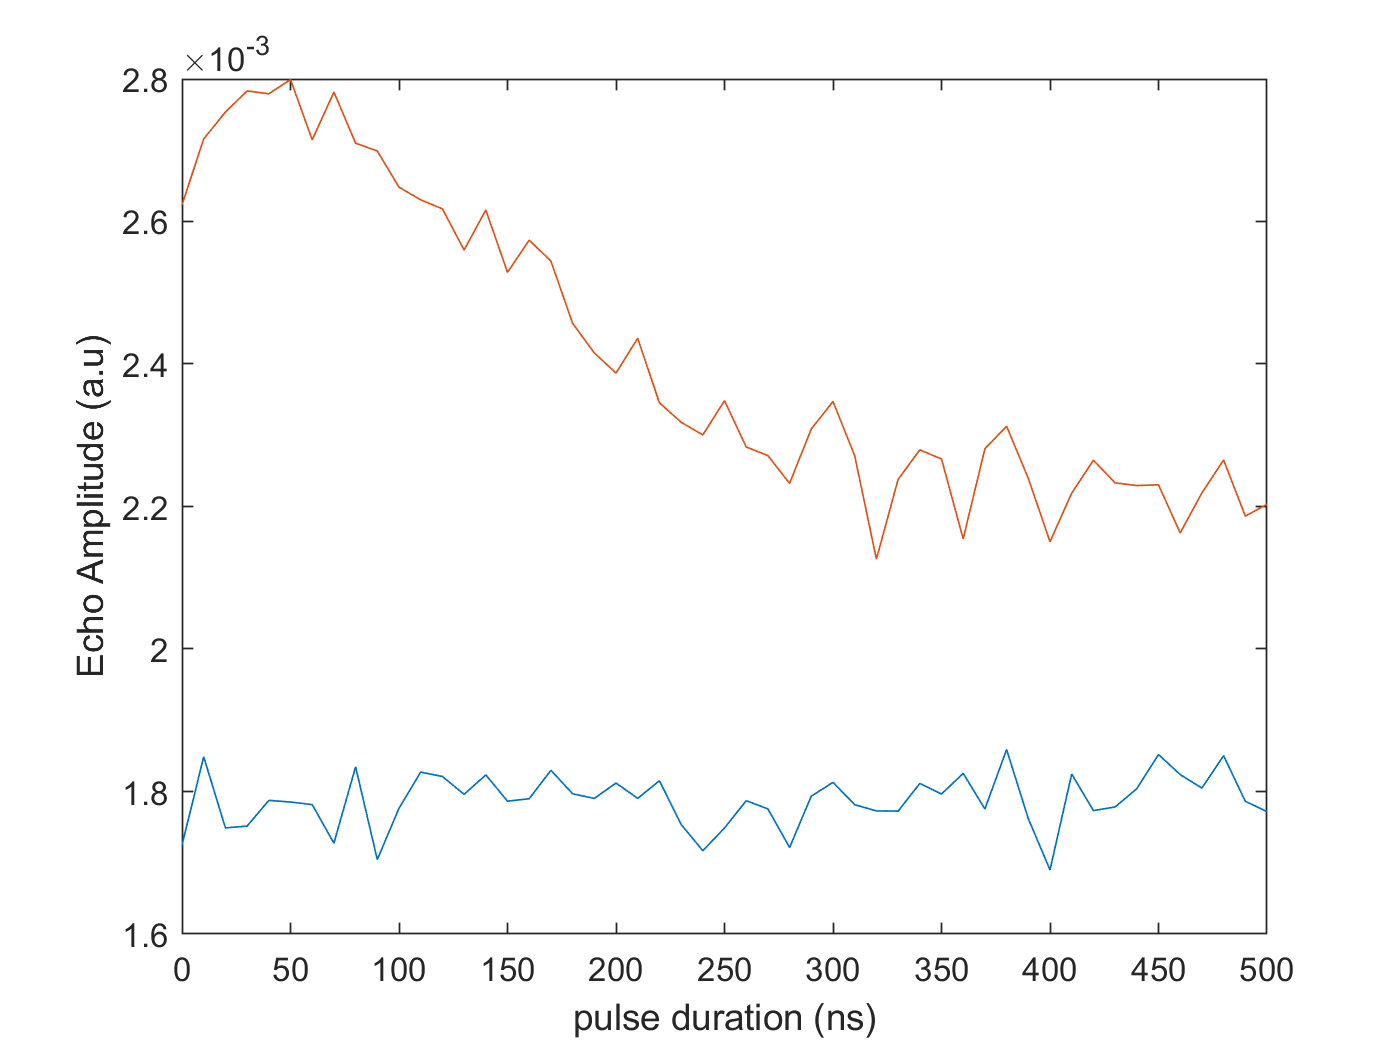
\includegraphics[width=\textwidth]{rabisi28}
        \caption{\label{fig:rabisi28}}
    \end{subfigure}
%     \hfill
    \begin{subfigure}[b]{0.45\textwidth}
        \centering
        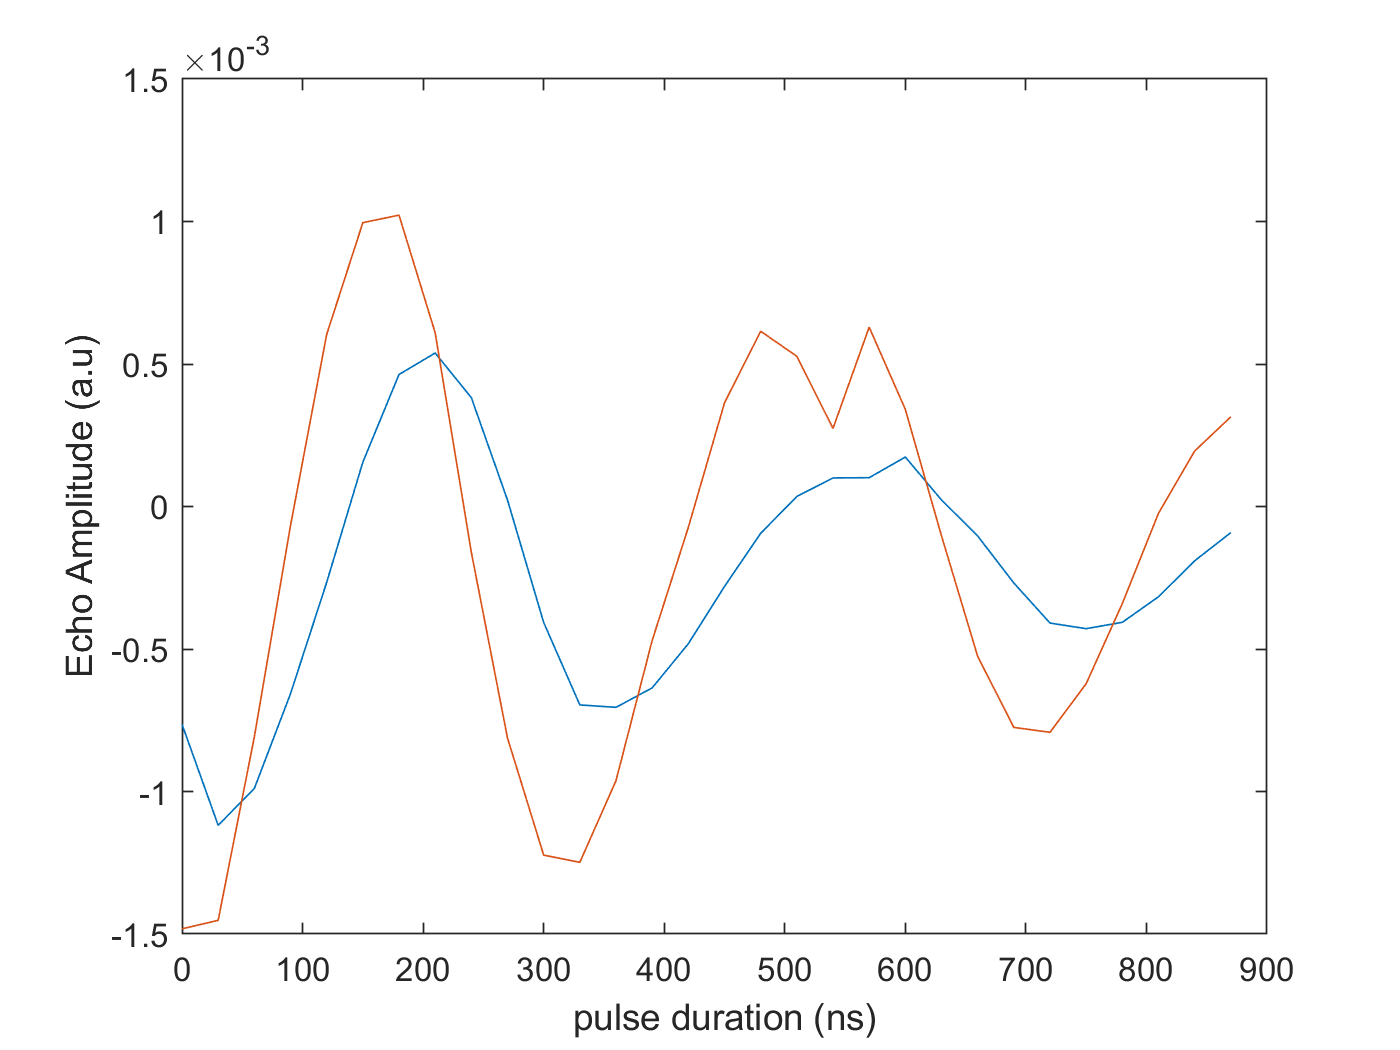
\includegraphics[width=\textwidth]{rabisinatural}
   \caption{\label{fig:rabisinatural}}
   \end{subfigure}
    \caption{Response to rabi pulse sequence of (a) $^28$Si doped with P and (b) natural Si doped P. The in-phase (I) and out-of-phase (Q) signals are shown in blue and red, respectively.}
\end{figure}

Due to concern that the issue was the significant fluctuations of the magnetic field during measurement since the field controller is normally constantly left running provide the most stable field, the sample was switched to a natural Si sample. The contribution of the $^{29}$Si nuclear spins results in dephasing which broadens the resonance linewidth~\citep{Hileeaaq1459}. The Rabi oscillations obtained for the natural Si sample is shown in Fig.~\ref{fig:rabisinatural}. An inversion recovery pulse sequence was completed to determine $T_{1}$ of $\approx 20$ ms.    

\section{$^{171}$Yb$^{3+}$:YSO EPR spectra}
The $^{171}$Yb$^{3+}$:YSO is then placed into the cryostat in approximate orientation of $B_{0}\parallel D1$ (or anti-parallel) in the $D1D2$ plane. The EPR transitions are probed at 7 K by sweeping the magnetic field sweeping based on the expected magnetic field resonance given in Fig.~\ref{fig:simmagresori3}. The linewidth of the site I and site II transitions are given as 3.4 mT and 0.1 mT~\citep{PhysRevB.97.064409}. The Q-factor of $\approx$385 is set to provide low energy damping but with a large enough frequency bandwidth to excite the spins. Upon detection of a site II echo pulse, similarly the Rabi experiment is completed to obtain for the amplitude of the AC signal used the optimum pulse duration of $\approx$70 ms to produce a $\pi$ rotation. 

The inversion recovery pulse sequence obtains $T_{1}\approx$2.6 ms which is in good agreement with the expected value at 7 K given in Fig.~\ref{fig:spinrelaxation}. $T_{2}$ is measured as $\approx 9$ $\mu$s using the Hahn echo detection pulse scheme. The measured echo signal for each of the three experiments is given in Appendix~\ref{sec:additionalresults} which is considerably more noisy than in Fig.~\ref{fig:rabisi28} and Fig.~\ref{fig:rabisinatural} due having to remove averaging of the echo signal due to this causing the oscilloscope to continually become unresponsive. However single-shot echo detection, as shown in Fig.~\ref{fig:cleanecho} is adequate for the purposes of this experiment. 

\section{\label{sec:strainexp}$^{171}$Yb$^{3+}$:YSO strain investigation}

Initially the strategy to investigate the effect of strain was to measure the Hahn echo signals whilst increasing mass is placed on top of the sample, applying unaxial stress along the b-axis. The shift in the resonance frequency can then be extracted by fitting to the echo represented in Fourier space~\citep{PhysRevLett.120.167701}. However, upon testing this method concerning observation was made, when a mass was placed on the rotation plane the echo signal completely vanished regardless of the mass used. Therefore, it was clear the shift in the resonance was the result of another mechanism determined to be crystal rotation. Due to the measured sensitivity of the magnetic field resonances to angular rotation of the crystal. The crystal was purposefully rotated 40$^{\circ}$ to approximately 140$^{\circ}$ or 320$^{\circ}$ as shown in Fig.~\ref{fig:site2D1inD1D2plane} (and Fig.~\ref{fig:site2D1inD1D2plane}). However, even for this crystal orientation the sensitivity to a small ($\approx 1-2^{\circ}$) rotation results in a significant shift of the resonance transition. 

\begin{figure}[H]
    \centering
    \begin{subfigure}[b]{0.45\textwidth}
        \centering
        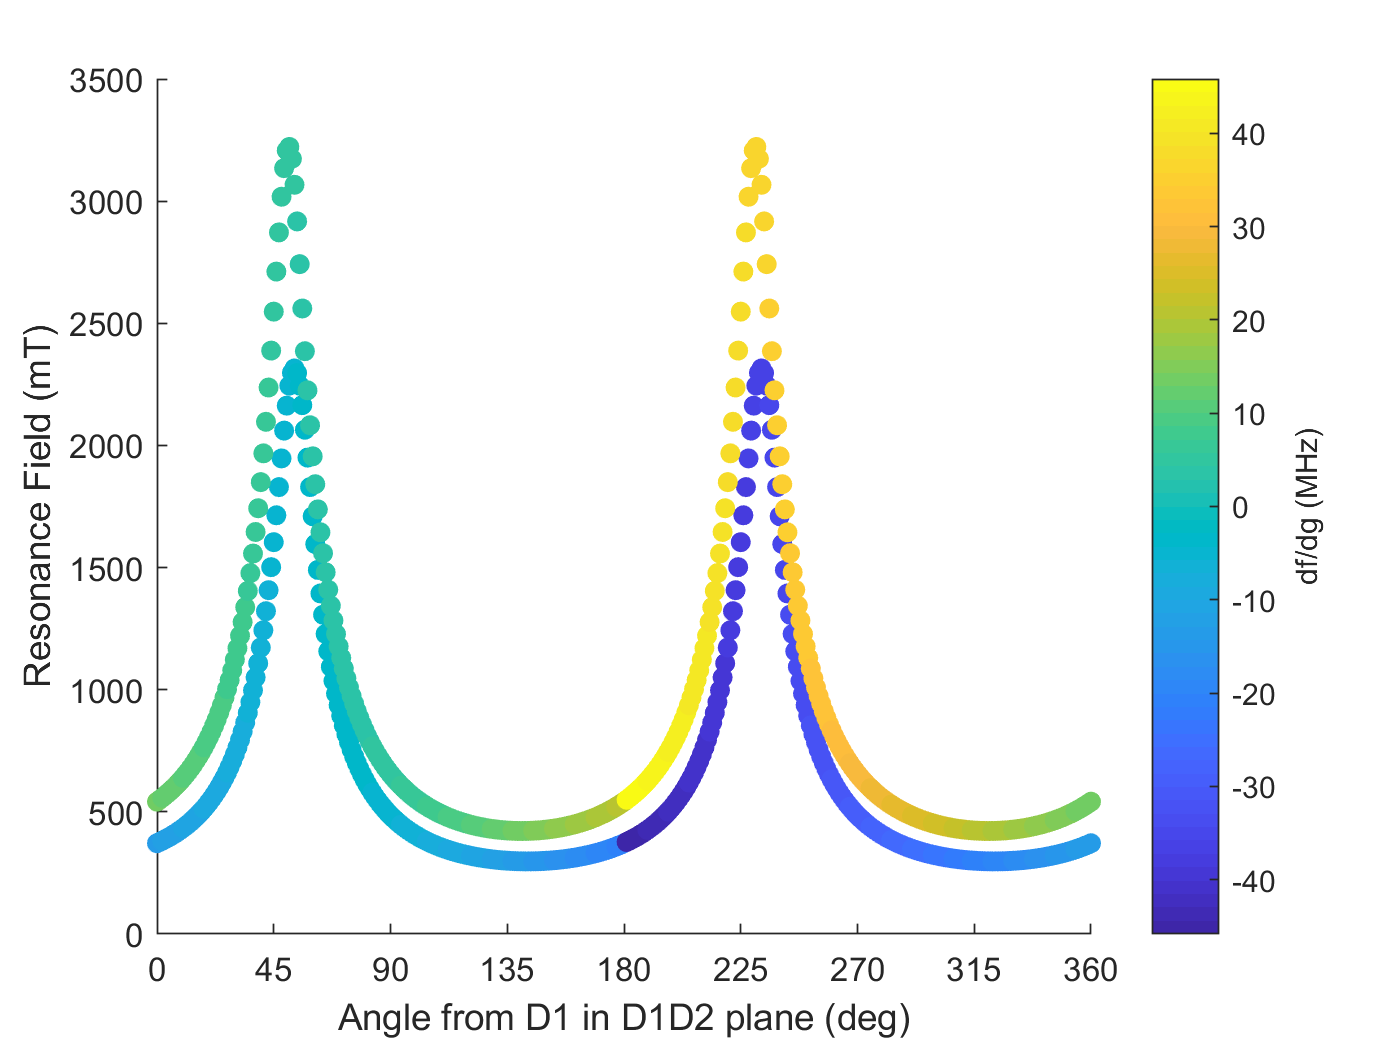
\includegraphics[width=\textwidth]{site2D1inD1D2plane}
        \caption{\label{fig:site2D1inD1D2plane}}
    \end{subfigure}
%     \hfill
    \begin{subfigure}[b]{0.45\textwidth}
        \centering
        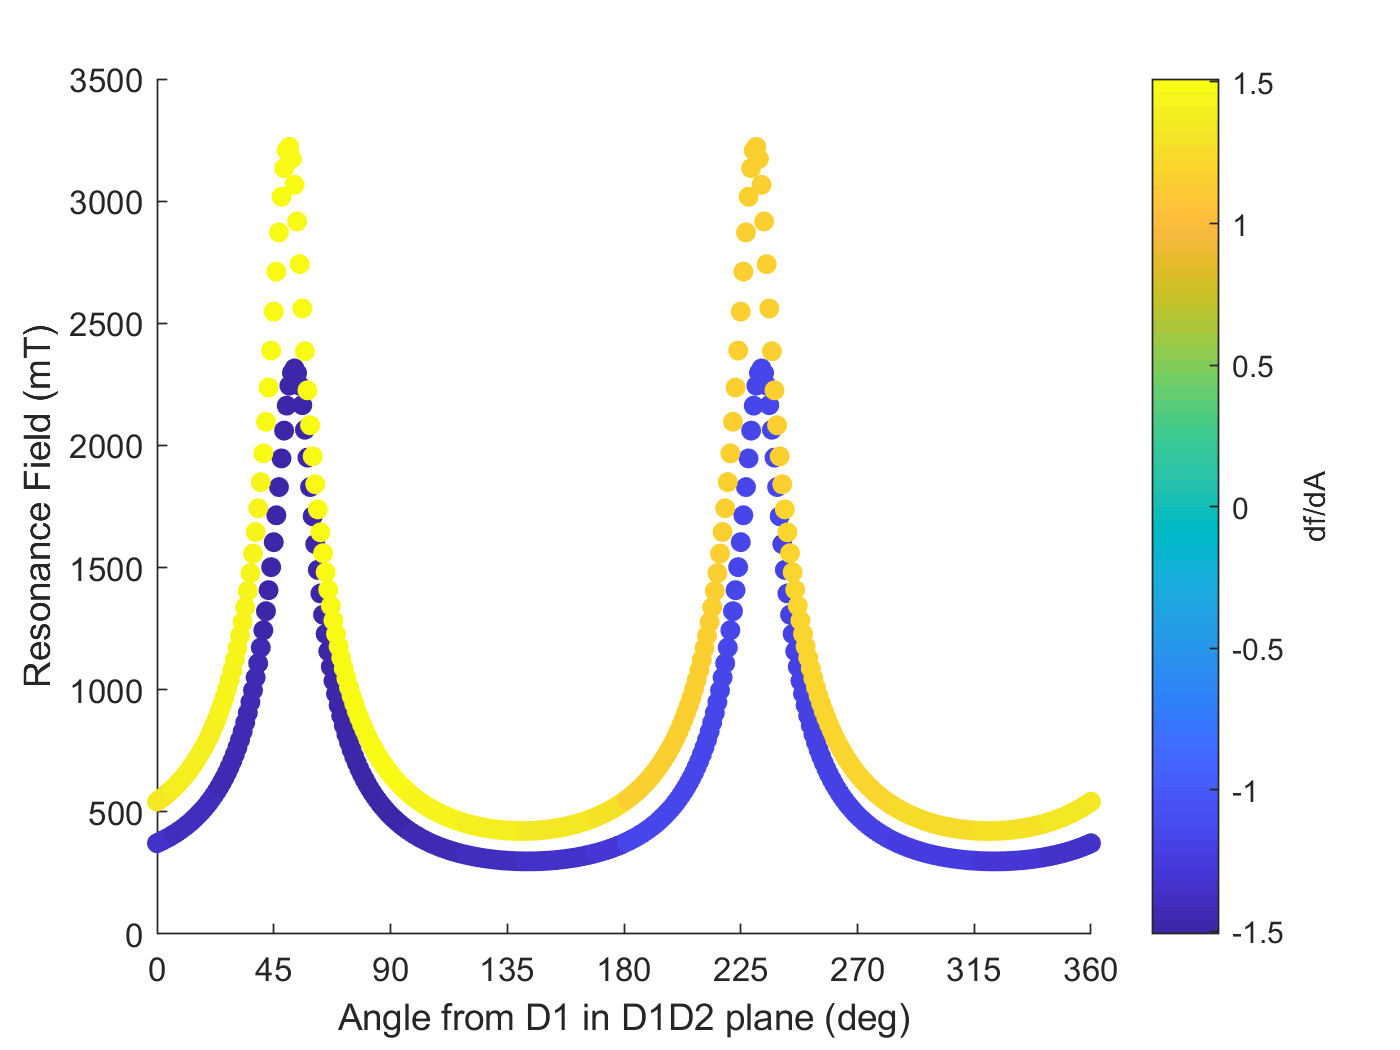
\includegraphics[width=\textwidth]{site2D1inD1D2planeA}
   \caption{\label{fig:site2D1inD1D2planeA}}
   \end{subfigure}
       \begin{subfigure}[b]{0.45\textwidth}
        \centering
        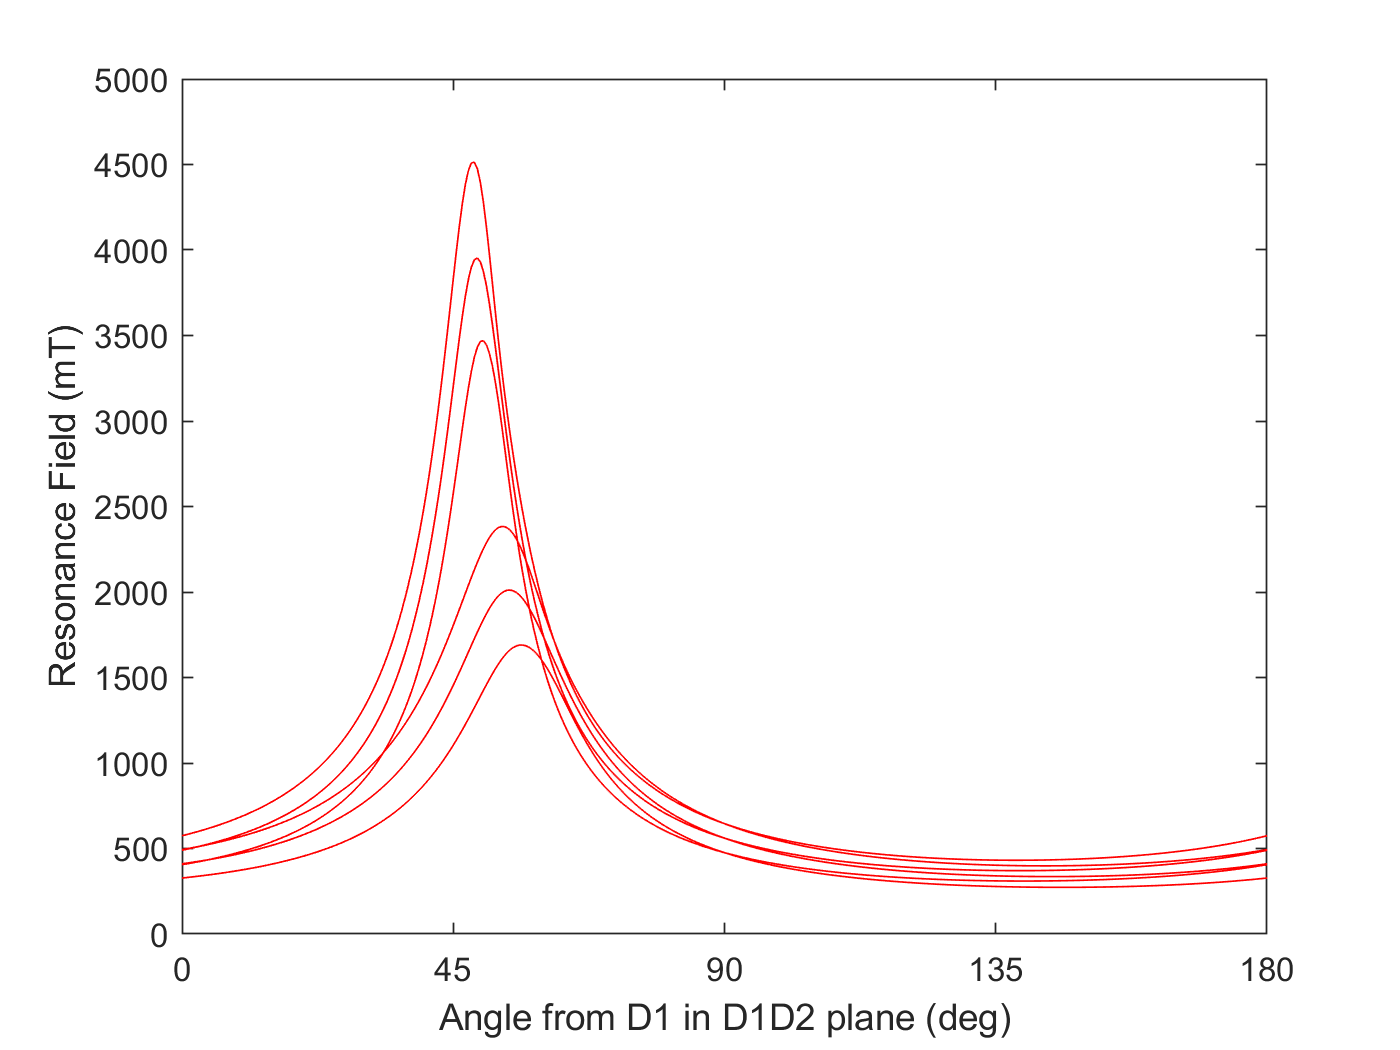
\includegraphics[width=\textwidth]{straininducedsplittingeasyspin}
   \caption{\label{fig:straininducedsplittingeasyspin}}
   \end{subfigure}
    \caption{Angular variations of the EPR transitions for site II $^{171}$Yb:YSO, where $\bm{B_{0}}$ is perpendicular the b-axis. The colour bar represents (a) $\Delta f/\Delta g$ for isotropic $\Delta g = 0.05$ and (b) $\Delta f/\Delta A$ for isotropic $\Delta A = 50$ MHz. (c) The 
    .}
\end{figure}

Therefore an alternative measurement approach was adopted. The magnetic field strength was swept over the region of the expected site II transitions for each additional mass stacked on top of the rotation plate. The transition detected for the initial $B_{0}$ sweep where the only applied strain is due to the weight of the sample rod in Fig.~\ref{fig:strainexpfirstfieldsweep} where six sharp peaks are detected. For due to the two-fold axis symmetry for this orientation the expectation is four site II EPR transitions. The additional measured peaks may be due to additional RE isotopes being present in the sample or weak amplitude forbidden $\Delta m_{I} = \pm 1$ transitions~\citep{PhysRevB.97.064409}. Comparison of experimental resonances to Fig~\ref{fig:straininducedsplittingeasyspin} where all site II transitions, including the forbidden transitions, are shown. Matching between the experimental and simulated EPR resonances determines the orientation in the $D1D2$ is $\theta = 120.5\pm 12.4^{\circ}$. If strain induces a dominant shift in the A-tensor then for the $m_{I}=0$ resonances the relative spacing between peaks is expected to change. However, if strain induces a shift in the g-tensor then the resonances are expected to shift in unison with an unaltered relative peak position. Fig.~\ref{fig:strainexpfirst1} presents shift in the EPR transitions as a function of the largest strain component is $\epsilon_{3}$ when unaxial stress ($\sigma_{3}$) is applied along the b-axis.     

\begin{figure}[H]
    \centering
    \begin{subfigure}[b]{0.45\textwidth}
        \centering
        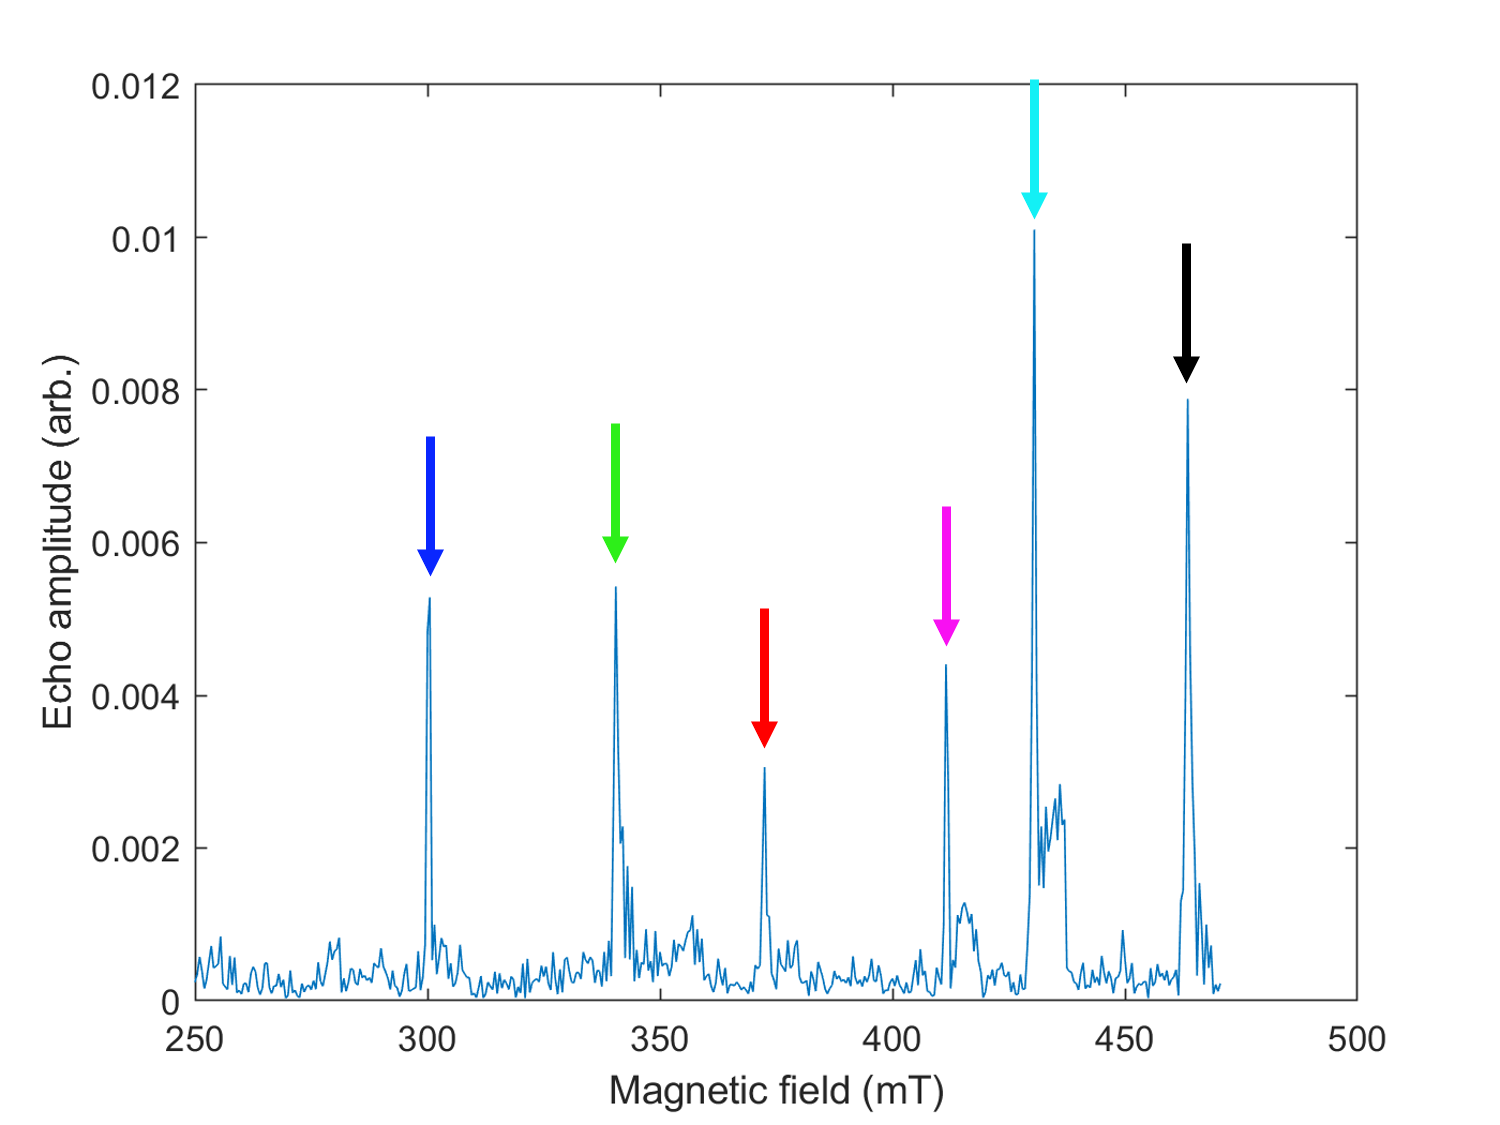
\includegraphics[width=\textwidth]{strainexpfirstfieldsweep}
        \caption{\label{fig:strainexpfirstfieldsweep}}
    \end{subfigure}
%     \hfill
    \begin{subfigure}[b]{0.45\textwidth}
        \centering
        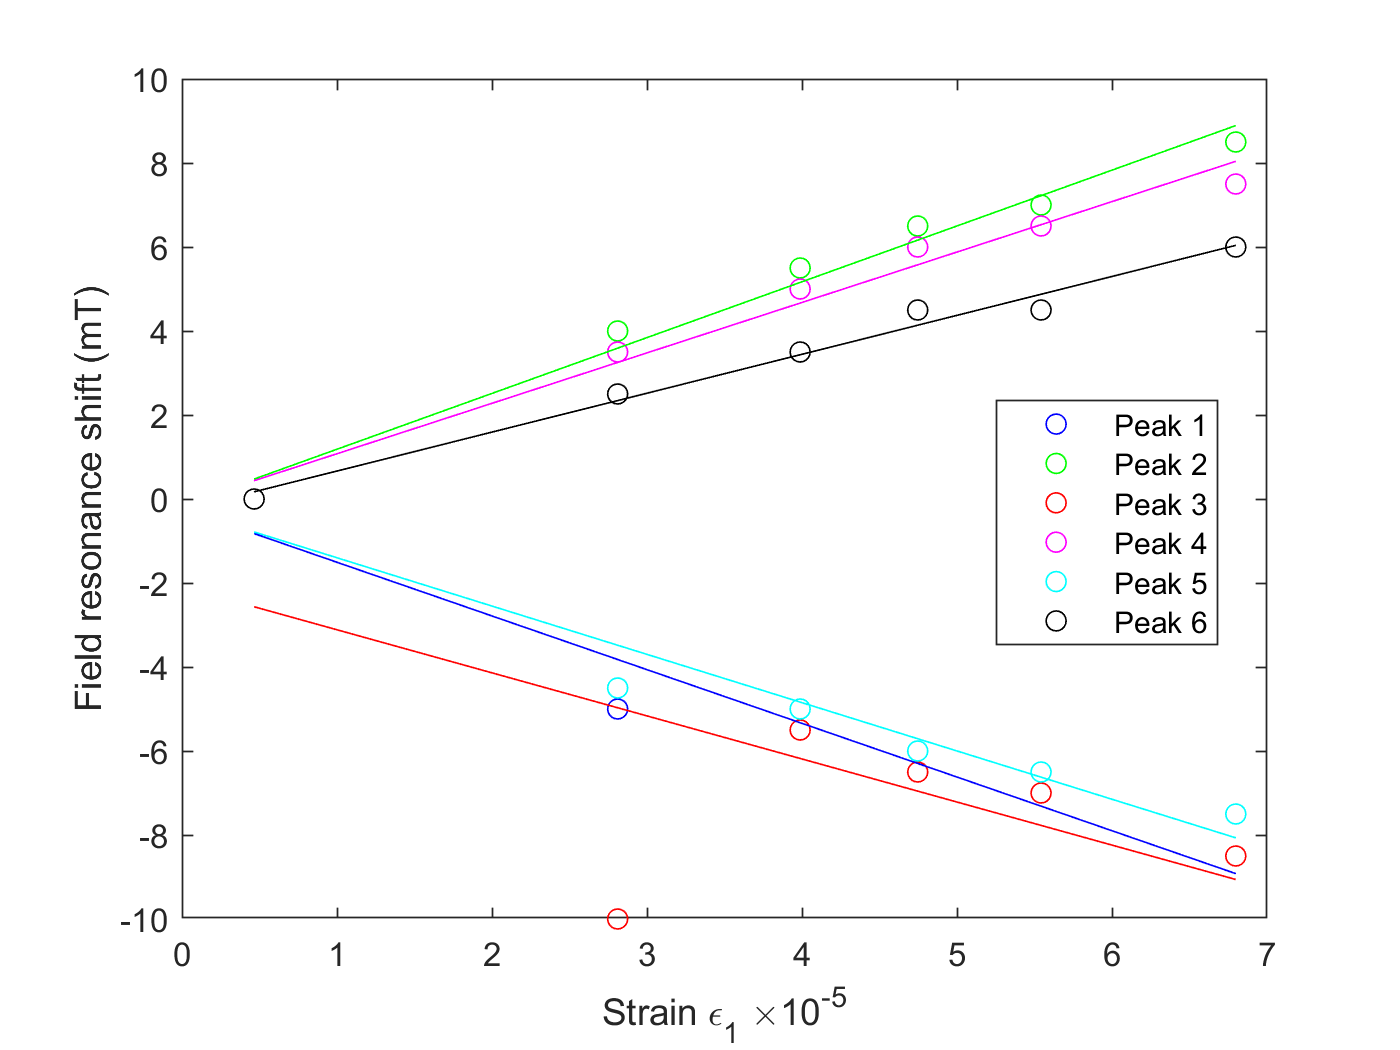
\includegraphics[width=\textwidth]{strainexpfirst1}
   \caption{\label{fig:strainexpfirst1}}
   \end{subfigure}
   \caption{(a) Magnetic field sweep over EPR transitions in site II with no mass on the rotation plate. (b) Magnetic resonance shift as a function of $\epsilon_{3}$ with applied linear fits. The sample orientation, $\theta$ = 120.5$\pm 12.4 ^{\circ}$ (or 300.5$\pm 12.4^{\circ}$) from $D1$ in the $D1D2$ plane.}
\end{figure}

Clipping of the echo signal was observed during the measurement of the data displayed in Fig.~\ref{fig:strainexpfirstfieldsweep}. Therefore, the function controlling the dynamic voltage range of the oscilloscope was modified such that the echo signal was no longer clipping. The experiment was repeater with finer sweeping around the resonances detected in the initial field sweep in Fig.~\ref{fig:strainexpsecondfieldsweep}. Lorentzian fitting of EPR resonances is completed as shown in Fig~\ref{fig:0gfittingpeaks} to obtain the peak amplitude, linewidth and resonance field values. Similarly the initial sample orientation is probed by comparing the EPR transitions in Fig.~\ref{fig:strainexpsecondfieldsweep} to Fig.~\ref{fig:straininducedsplittingeasyspin} although in this case a mass of 504 g is initially placed on the rotation plate. For the largest magnetic field resonance transition ($\ket{S=1/2,m_{I}=1/2} \leftrightarrow \ket{S=-1/2,m_{I}=1/2}$) shown by the black arrow in Fig.~\ref{fig:strainexpsecondfieldsweep} there is no site II orientation such that this EPR transition has a value below 430 mT. Therefore this could be an indicator that the strain has shifted the resonance. The ($\ket{S=1/2,m_{I}=-1/2} \leftrightarrow \ket{S=-1/2,m_{I}=-1/2}$) transition in green in Fig.~ref{fig:strainexpsecond1} appears to be insensitive to small changes of sample orientation such that orientation is $\theta =139.5 \pm 4^{\circ}$ (or 319.5$\pm 4^{\circ}$).          

\begin{figure}[H]
    \centering
    \begin{subfigure}[b]{0.45\textwidth}
        \centering
        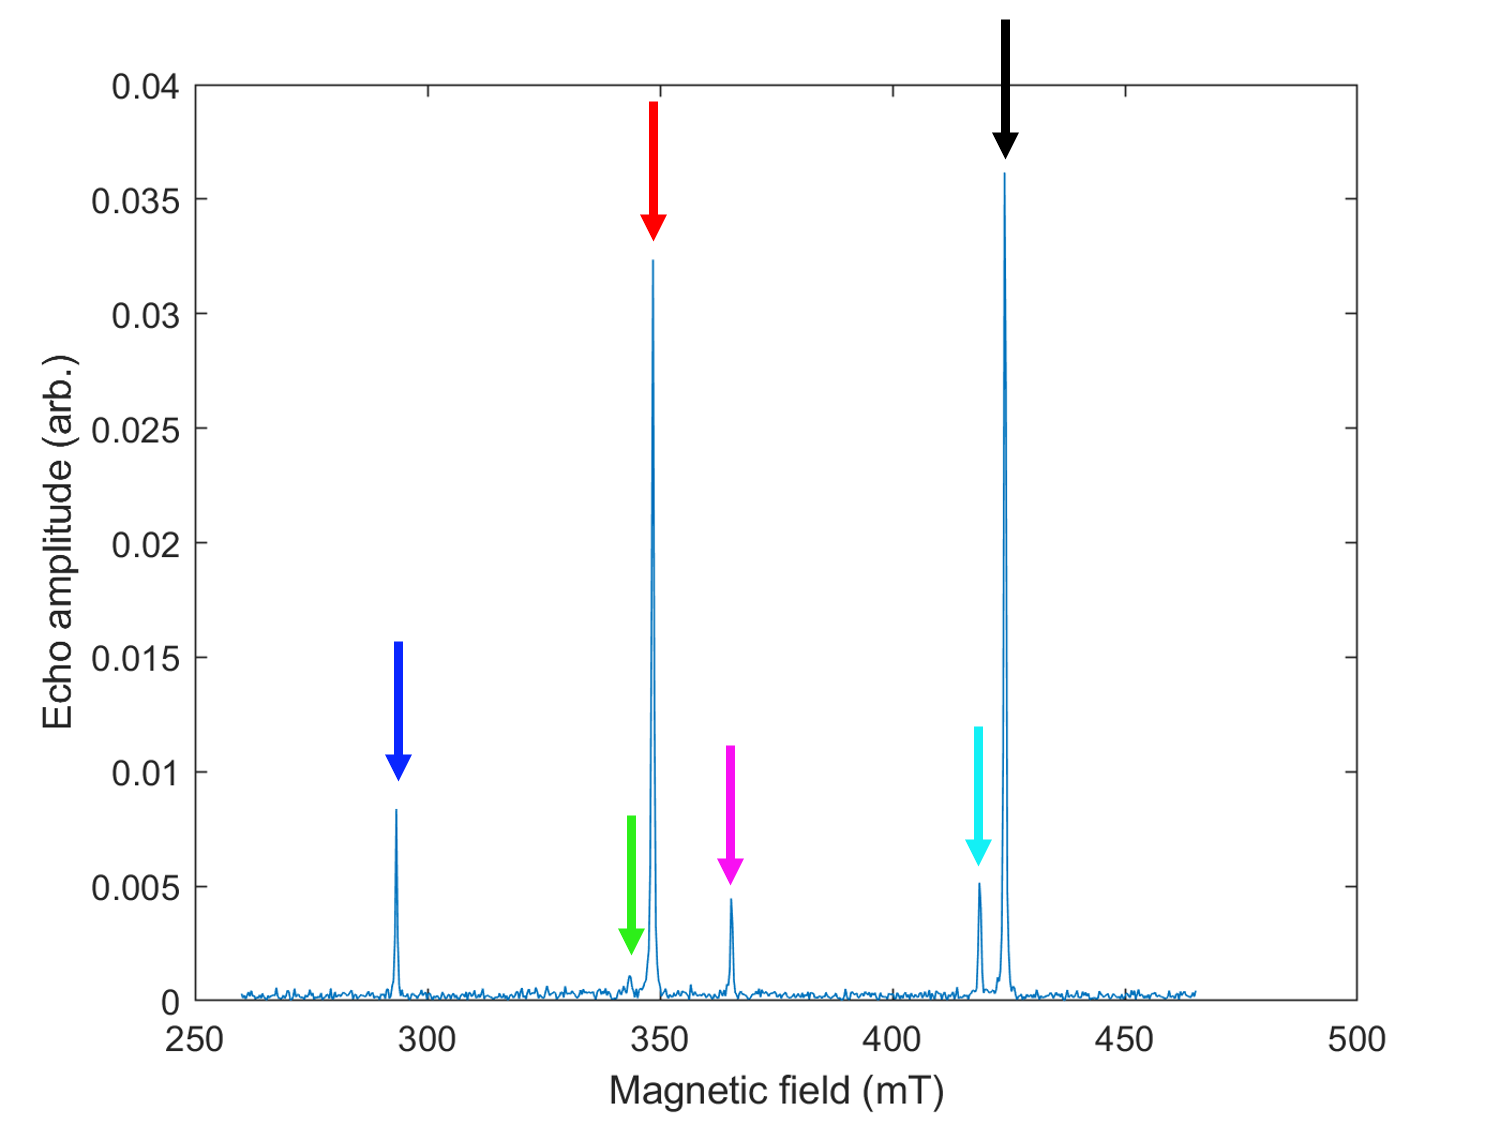
\includegraphics[width=\textwidth]{strainexpsecondfieldsweep}
        \caption{\label{fig:strainexpsecondfieldsweep}}
    \end{subfigure}
%     \hfill
    \begin{subfigure}[b]{0.45\textwidth}
        \centering
        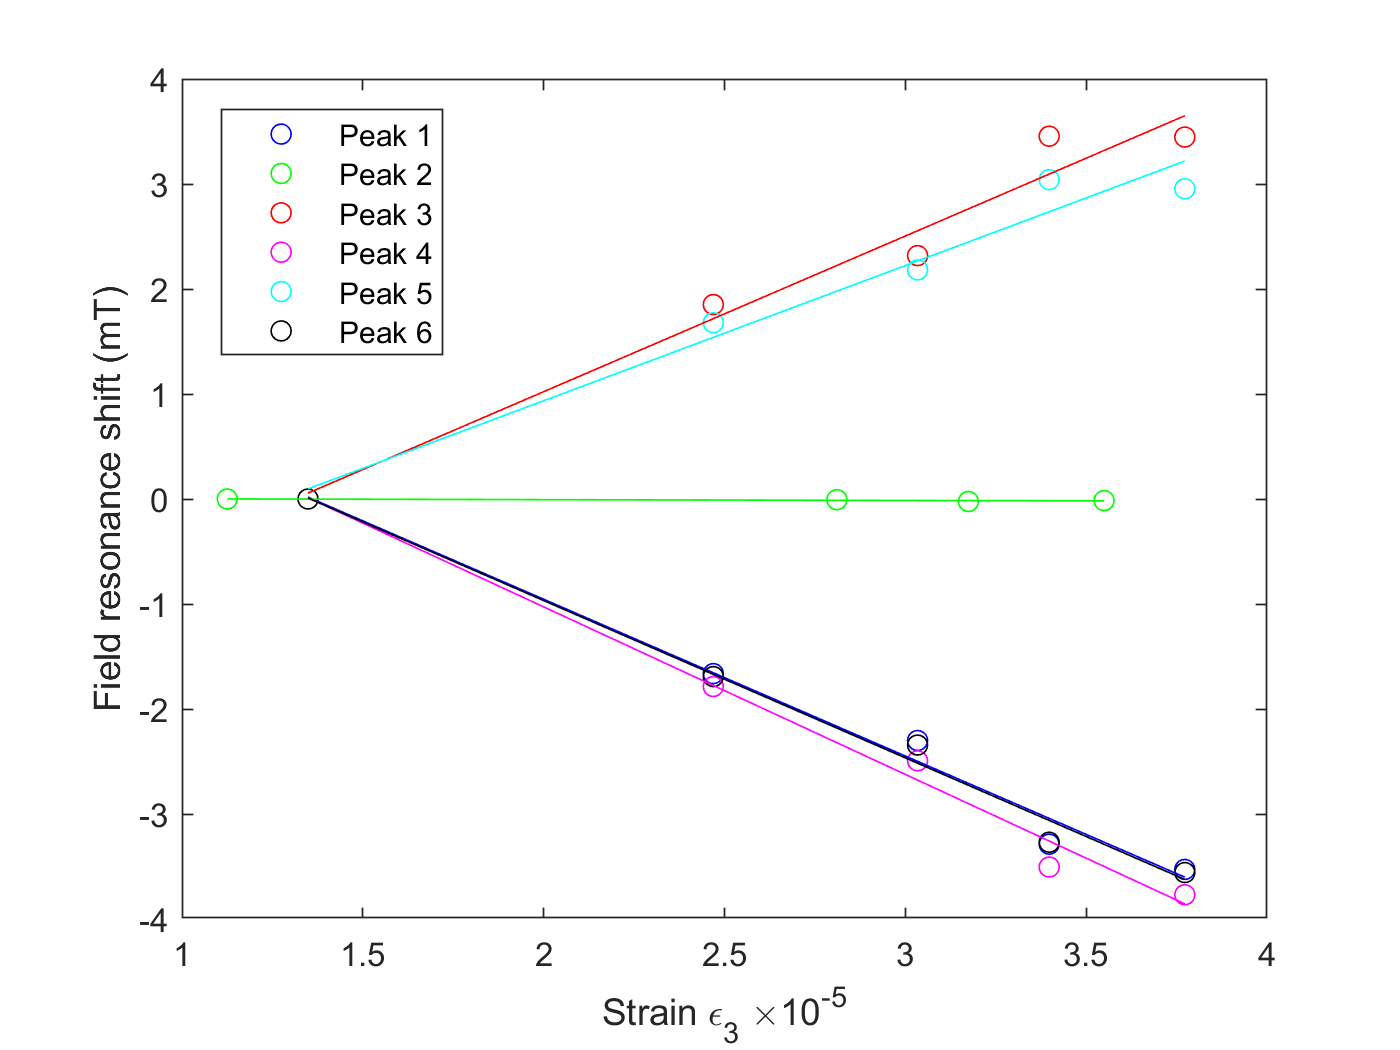
\includegraphics[width=\textwidth]{strainexpsecond1}
   \caption{\label{fig:strainexpsecond1}}
   \end{subfigure}
       \begin{subfigure}[b]{0.45\textwidth}
        \centering
        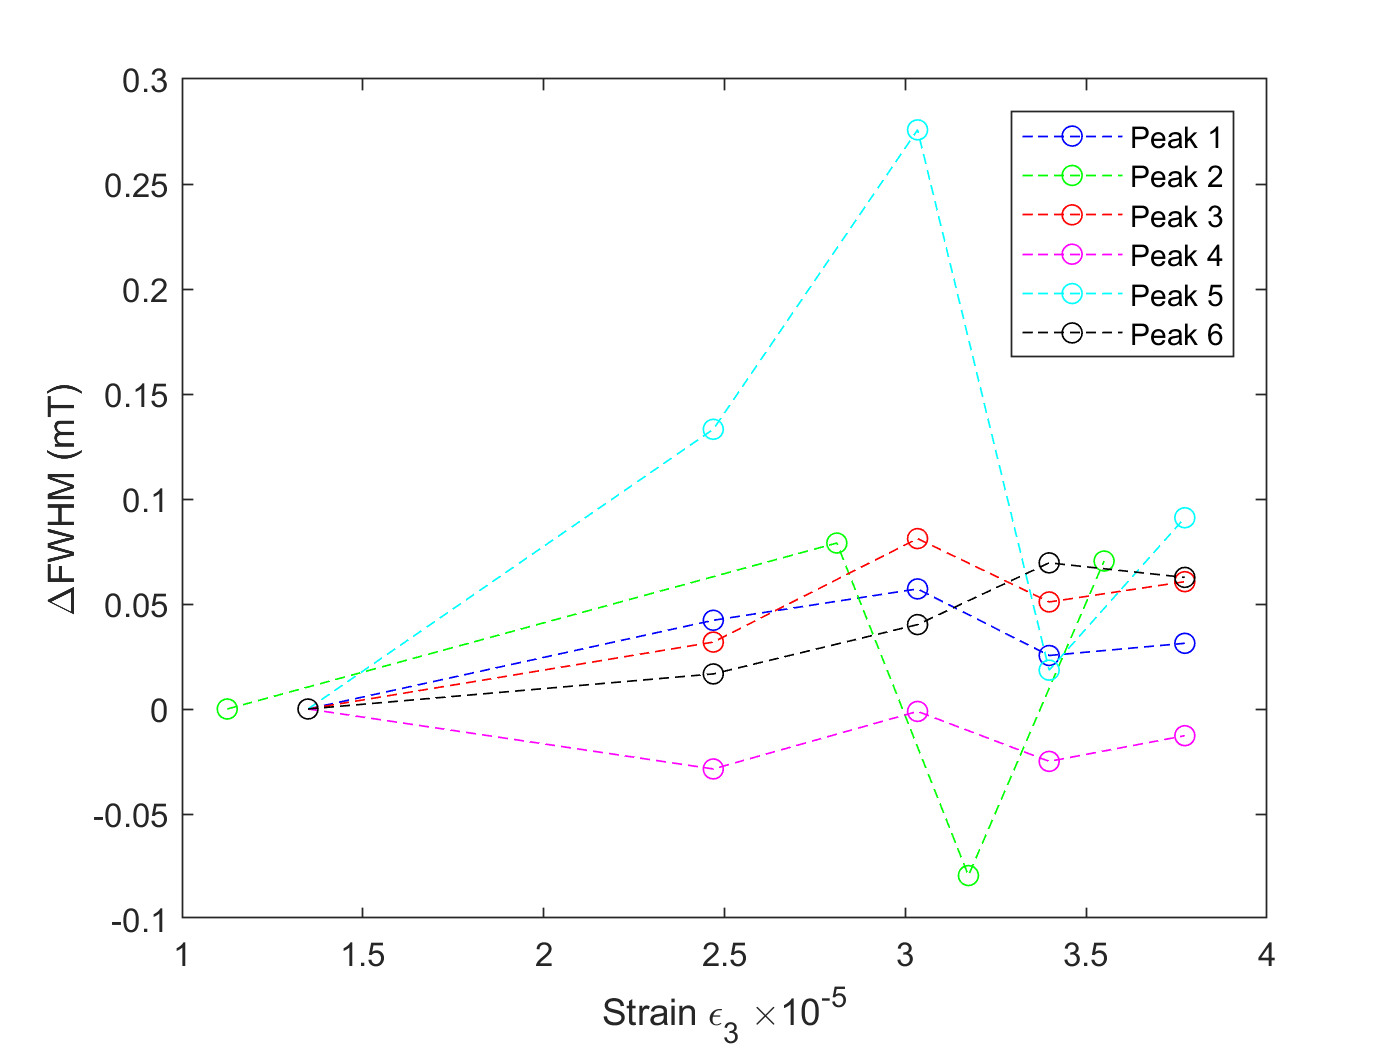
\includegraphics[width=\textwidth]{strainexpsecond2}
   \caption{\label{fig:strainexpsecond1}}
   \end{subfigure}
       \begin{subfigure}[b]{0.45\textwidth}
        \centering
        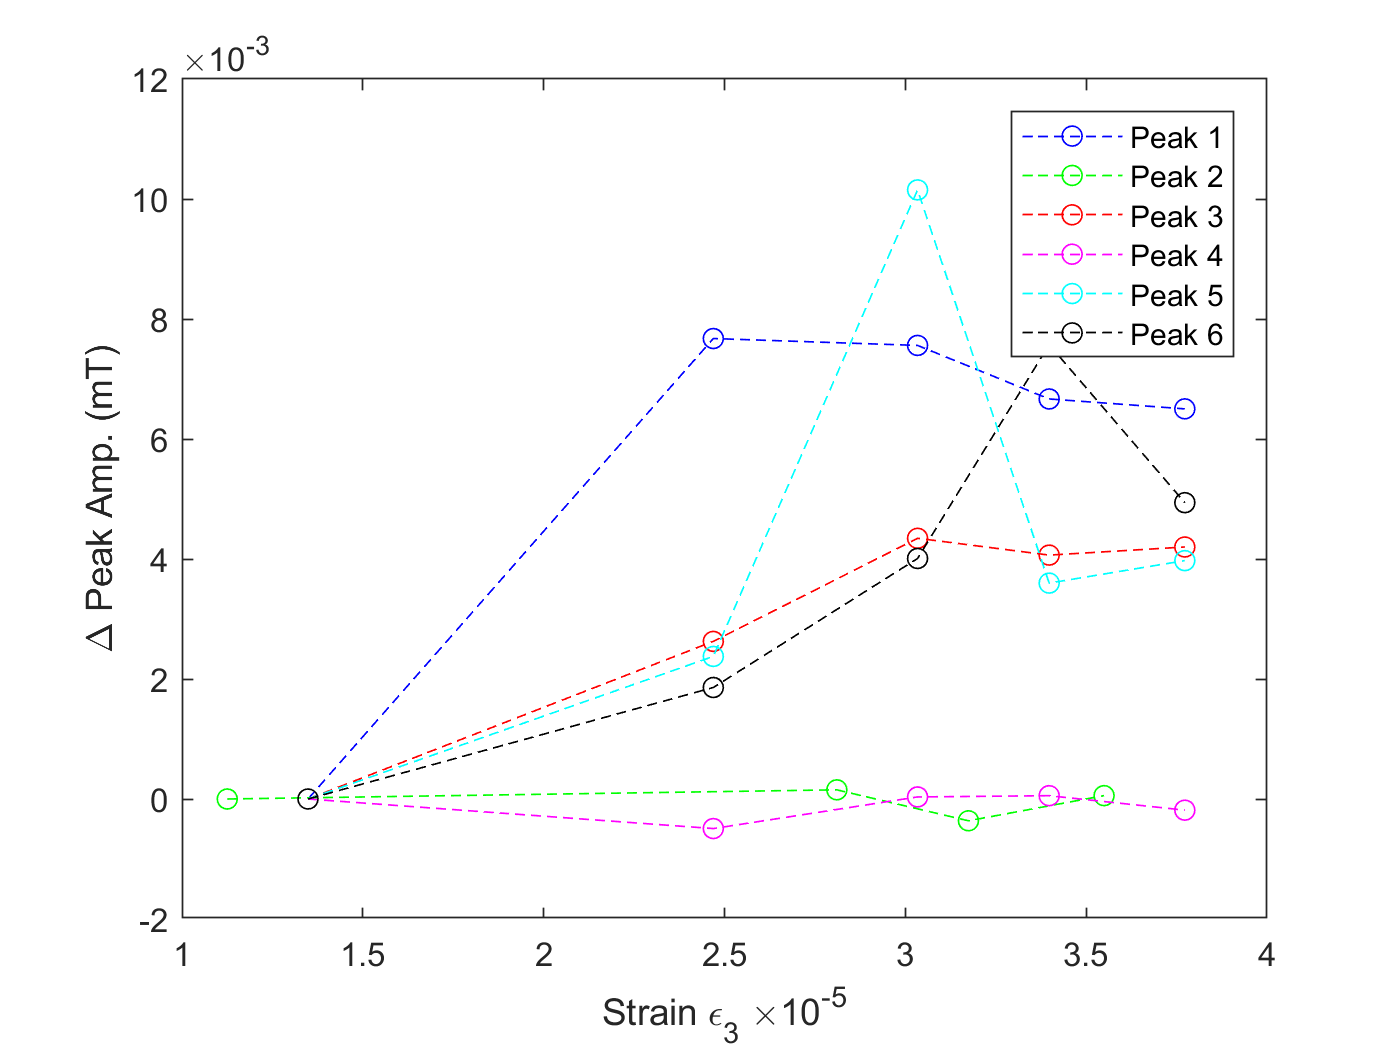
\includegraphics[width=\textwidth]{strainexpsecond3}
   \caption{\label{fig:strainexpsecond1}}
   \end{subfigure}
   \caption{Yb:YSO site II EPR transitions for $\theta$ = 139.5$\pm 4^{\circ}$ (or 319.5$\pm 4^{\circ}$) from $D1$ in the $D1D2$ plane. (a) Magnetic field sweep over EPR transitions with 504 g mass initially on the rotation plate. (b) Magnetic resonance shift as a function of $\epsilon_{3}$ with applied linear fits. (c) Change in the EPR linewidth (full width half maximum FWHM) vs. $\epsilon_{3}$. (d) Change in the resonance signal amplitude vs. $\epsilon_{3}$.}
\end{figure}

Next the sample was rotated by 180$^{\circ}$ since for a small perturbation of $\bm{A}$ on sample orientation with respect to the $B_{0}$ generates a larger value of $df/dA$. The magnetic field sweep in Fig.~\ref{fig:strainexpthirdfieldsweep} revealed an additional weak echo signal. As expected the apparent insensitivity of the red transition peak of Fig.~\ref{fig:strainexpthird1} is used to determine sample orientation of $\theta=$319.5$\pm 4^{\circ}$ (or $139.5 \pm 4^{\circ}$). Measured approximately linear shift of the resonance field as $\epsilon_{3}$ is increased is shown in Fig.~\ref{fig:strainexpthird1} where the additionally cross markers display the measurements as the masses are removed from the rotation plate. The all resonances shift significantly, excluding peak 3, as the masses are removed which is expected to be the product of unwanted sample rotation. 

\begin{figure}[H]
    \centering
    \begin{subfigure}[b]{0.45\textwidth}
        \centering
        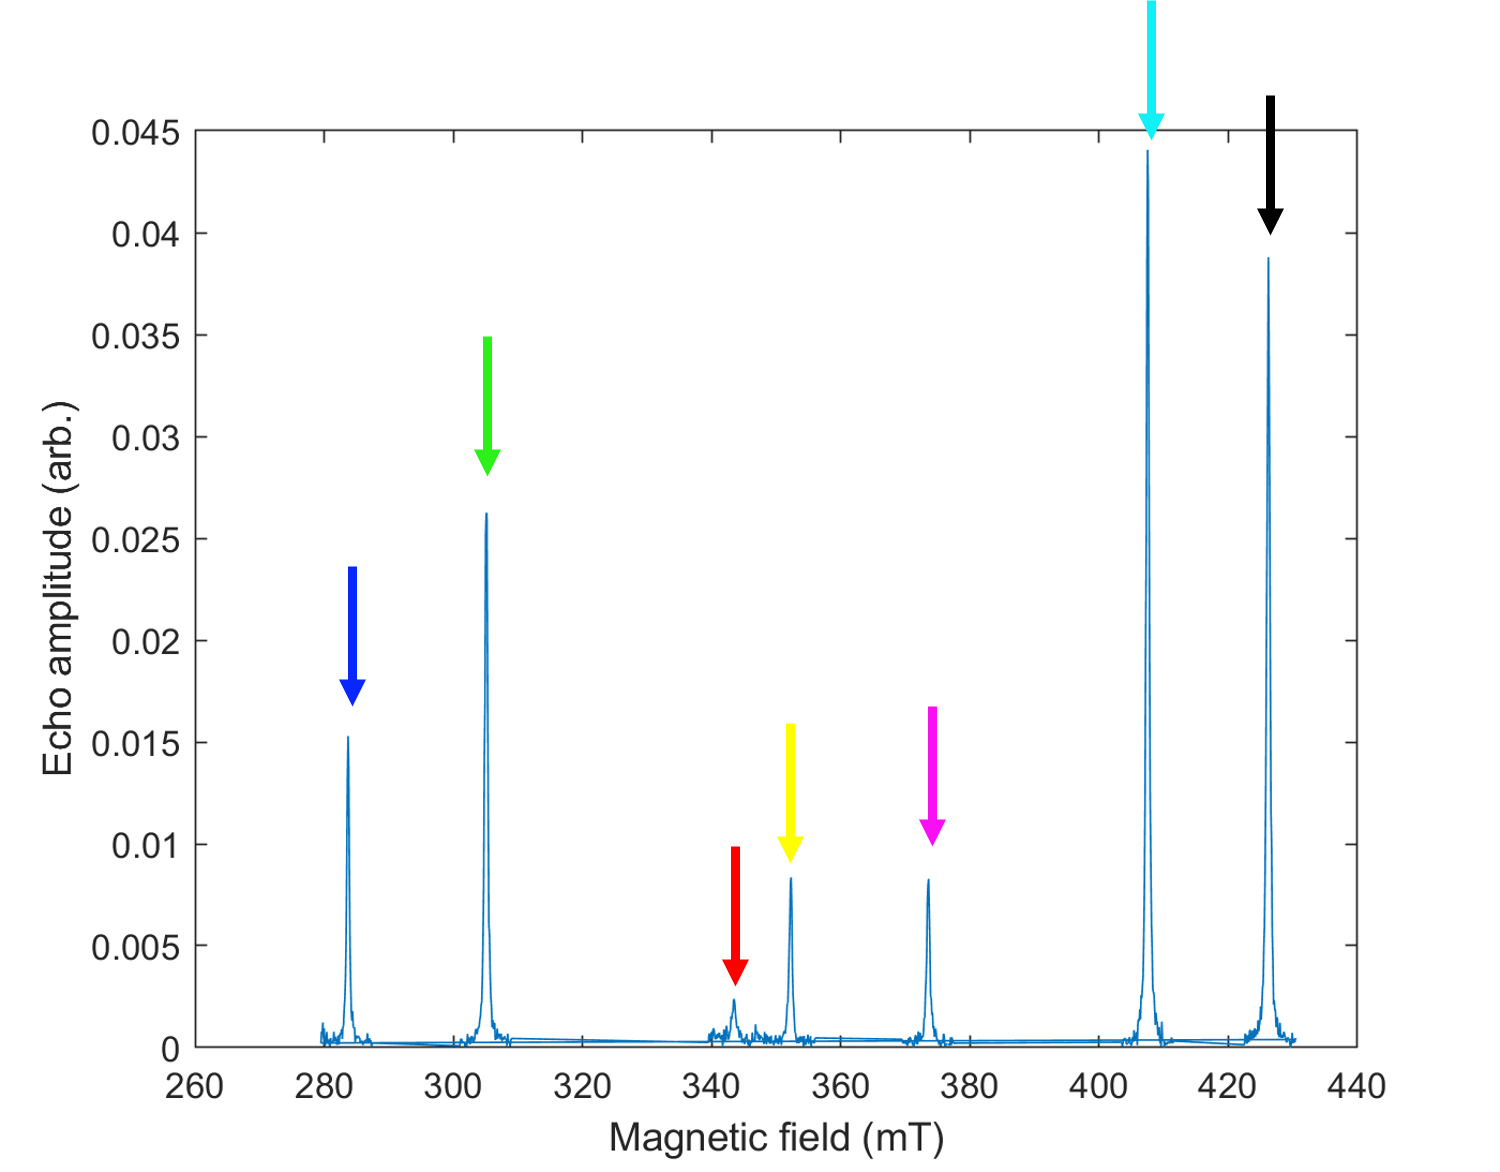
\includegraphics[width=\textwidth]{strainexpthirdfieldsweep}
        \caption{\label{fig:strainexpthirdfieldsweep}}
    \end{subfigure}
%     \hfill
    \begin{subfigure}[b]{0.45\textwidth}
        \centering
        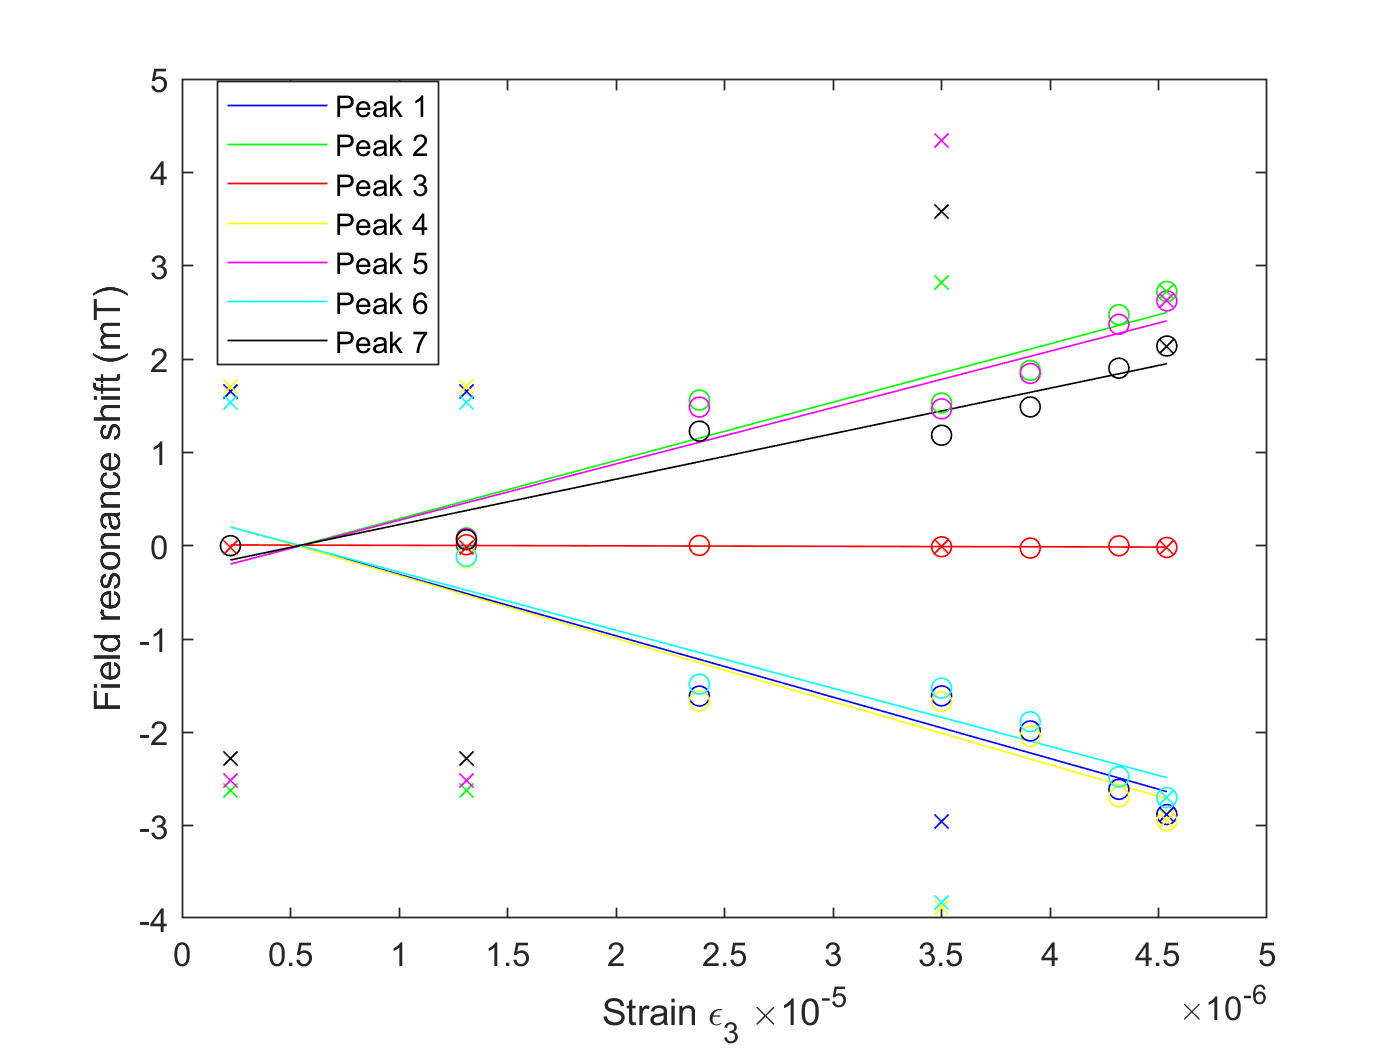
\includegraphics[width=\textwidth]{strainexpthird1}
   \caption{\label{fig:strainexpthird1}}
   \end{subfigure}
   \caption{Yb:YSO site II EPR transitions for $\theta$ = 139.5$\pm 2^{\circ}$ (or 319.5$\pm 2^{\circ}$) from $D1$ in the $D1D2$ plane. (a) Magnetic field sweep over EPR transitions with 504 g mass initially on the rotation plate. (b) Magnetic resonance shift as a function of $\epsilon_{3}$ with applied linear fits.}
\end{figure}









